\chapter{Introduction}
\label{chap:intro}
\lhead{Chapter \ref{chap:intro}. \emph{\nameref{chap:intro}}} % This is for the header

In recent years, there has been a large increase in both the quantity and availability of geographic data. This new surge of such large quantities of data has prompted a similar rise on the number of applications to capture, store, manipulate and analyse this data.
A lot of these applications share the need to visualise the geographic information in such a way that it can be easily understood by a human.
This is usually done by displaying points of interest on a map so that their relative position or direction can be easily interpreted without much thought by the user.

One obstacle when representing large amounts of geographic data is that the sheer number of points to display can be overwhelming for a human, as well as computationally intensive to render for a machine. As such, there is a need to develop and implement a viable way to reliably calculate and display a subset of geographic points, whilst keeping a degree of representability of the larger set, so that as little information as possible is absent when the representative subset is shown.

The purpose of this project is to research and develop a real-time algorithm that can analyse geographic data provided by a geographic information system (GIS) infrastructure developed and maintained at Smartgeo. More precisely, the developed algorithm will have to be able to aggregate and select geographic points according to a given a set of criteria. Figure \ref{fig:rep} shows an example of a representative subset of an original, larger set.
\begin{figure}[H]
	\centering
	\begin{minipage}{0.4\linewidth}
		\centering
		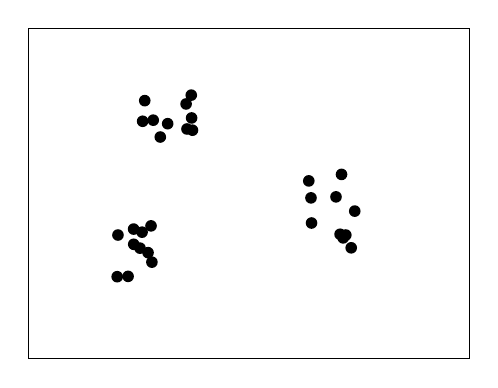
\begin{tikzpicture}[scale=1.4]
			\draw (-0.5,-0.4) rectangle (3.5,2.6);
			
			\fill (0.456,0.778)circle (1.5pt);
			\fill (0.622,0.478)circle (1.5pt);
			\fill (0.457,0.64)circle (1.5pt);
			\fill (0.614,0.807)circle (1.5pt);
			\fill (0.314,0.724)circle (1.5pt);
			\fill (0.533,0.75)circle (1.5pt);
			\fill (0.514,0.605)circle (1.5pt);
			\fill (0.307,0.346)circle (1.5pt);
			\fill (0.406,0.349)circle (1.5pt);
			\fill (0.587,0.564)circle (1.5pt);
			
			\fill (2.065,1.061)circle (1.5pt);
			\fill (2.045,1.215)circle (1.5pt);
			\fill (2.292,1.07)circle (1.5pt);
			\fill (2.381,0.724)circle (1.5pt);
			\fill (2.43,0.608)circle (1.5pt);
			\fill (2.342,1.274)circle (1.5pt);
			\fill (2.329,0.731)circle (1.5pt);
			\fill (2.462,0.941)circle (1.5pt);
			\fill (2.357,0.698)circle (1.5pt);
			\fill (2.07,0.833)circle (1.5pt);
			
			\fill (0.765,1.734)circle (1.5pt);
			\fill (0.557,1.943)circle (1.5pt);
			\fill (0.698,1.613)circle (1.5pt);
			\fill (0.634,1.766)circle (1.5pt);
			\fill (0.979,1.993)circle (1.5pt);
			\fill (0.99 ,1.675)circle (1.5pt);
			\fill (0.538,1.756)circle (1.5pt);
			\fill (0.932,1.913)circle (1.5pt);
			\fill (0.982,1.786)circle (1.5pt);
			\fill (0.94 ,1.686)circle (1.5pt);
		\end{tikzpicture}
		\caption*{\footnotesize Original Set}
		\label{fig:badrep}
	\end{minipage}
	\hspace{1cm}
	\begin{minipage}{0.4\linewidth}
		\centering
		\begin{tikzpicture}[scale=1.4]
		\draw (-0.5,-0.4) rectangle (3.5,2.6);
		
		\fill (0.765,1.734)circle (1.5pt);
		\fill (0.514,0.605)circle (1.5pt);
		\fill (2.292,1.07)circle (1.5pt);
		\end{tikzpicture}		
		\caption*{\footnotesize Representative Subset}
		\label{fig:goodrep}
	\end{minipage}
	\caption{Example of a Representative Set}
	\label{fig:rep}
\end{figure}

This thesis aims to research, develop, and analyse different algorithms to choose a representative subset of geographic points, whilst being able to dynamically change that set of points via zooming or panning over a geographic region containing a large amount of geographical data. In case the optimal solution algorithms prove to be too slow, heuristic approaches will be implemented. Heuristic algorithms will have their solution quality and speed benchmarked against implicit enumeration algorithms.
The algorithm that is deemed the best will be implemented in the web framework via the \emph{WFS} and \emph{WMS} web mapping standards.

This report is organized as follows:
Chapter \ref{chap:theory} - \nameref{chap:theory} defines the base theoretical concepts, such as a notion of representativeness, as well as some useful structures used in the algorithms. Chapter \ref{chap:sota} - \nameref{chap:sota} analyses previous related work. Chapter \ref{chap:algos} - \nameref{chap:algos} describes the implicit enumeration algorithms implemented so far, as well as an analysis on their time and space complexities. Chapter \ref{chap:approx} - \nameref{chap:approx} describes an approximation algorithm. 